\documentclass[tikz,border=12pt]{standalone}
\usepackage{fontspec}
\setmainfont{Segoe UI}
\usepackage{amsmath,amssymb}
\usepackage{tikz}

\usetikzlibrary{calc,arrows.meta}

\begin{document}
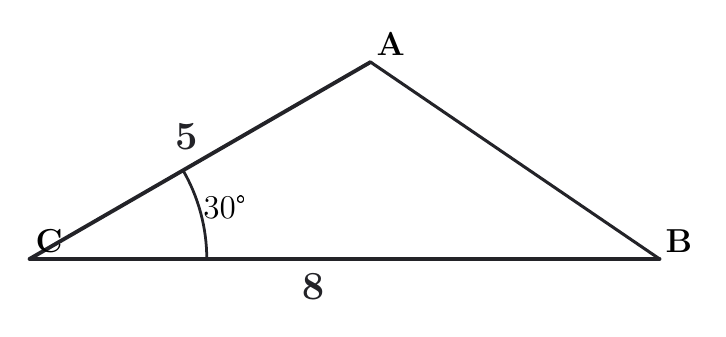
\begin{tikzpicture}[x=1.0000cm,y=1cm,line cap=round,line join=round]
\definecolor{linec0}{RGB}{35,35,40}
\definecolor{linec1}{RGB}{35,35,40}
\definecolor{linec2}{RGB}{35,35,40}
\definecolor{linec3}{RGB}{35,35,40}
\definecolor{linec4}{RGB}{35,35,40}
\definecolor{linec5}{RGB}{35,35,40}
\definecolor{edgecol}{RGB}{35,35,40}
\definecolor{hicol}{RGB}{35,35,40}
\definecolor{angcol}{RGB}{35,35,40}
\coordinate (C) at (0.0000,0.0000);
\coordinate (B) at (8.0000,0.0000);
\coordinate (A) at (4.3300,2.5000);
\draw[line width=1.4pt,color={rgb,255:red,35;green,35;blue,40}] (C) -- (B);
\draw[edgecol,line width=1.1pt] (B) -- (A);
\draw[line width=1.4pt,color={rgb,255:red,35;green,35;blue,40}] (A) -- (C);
\draw[edgecol,line width=1.00pt] (0.000,0.000)++(0.00:2.250) arc[start angle=0.00, delta angle=30.00, radius=2.250];
\node[text=black,font=\large] at (2.482,0.665) {30°};
\node[font=\bfseries\Large,text={rgb,255:red,35;green,35;blue,40}] at (3.600,-0.350) {8};
\node[font=\bfseries\Large,text={rgb,255:red,35;green,35;blue,40}] at (1.990,1.553) {5};
\node[font=\bfseries\large,inner sep=2pt,anchor=south west] at (0.000,0.000) {C};
\node[font=\bfseries\large,inner sep=2pt,anchor=south west] at (8.000,0.000) {B};
\node[font=\bfseries\large,inner sep=2pt,anchor=south west] at (4.330,2.500) {A};
\end{tikzpicture}
\end{document}
